\chapter{Adaptive function selection}
\label{chap:deciding}

The key purpose of the adaptive framework is to always invoke a function that is expected to have the best performance possible in a given environment and with given inputs. By \textit{function performance} we mean any measurable description of the qualities of the function. It can be the actual run time of the function, memory consumption, number of I/O operations, number of threads created, execution counts for various parts of the code, etc. All these factors can be valuable and be the goal of the system run optimization.

This thesis is focused on the task of optimizing the function run time or time complexity in general. The core of the framework, however, is designed to be extensible by modules that can analyze the function run in different ways. More on this topic will be covered in chapter \ref{chap:implementation}.

Note we will suppose some basic knowledge of mathematical statistics in this chapter. A nice introduction covering all the concepts that this text works with can be found in \cite{weiss_introductory_2010}.

\section{Overview of the selection process}
\label{sec:selection_overview}

Suppose we have functions $f_1,\dots, f_n$, all of them interchangeable, and an input $in$\footnote{If the original Scala function has multiple arguments \inlinecode{arg1, ..., argN}, we will consider them to be a tuple \inlinecode{(arg1, ..., argN)} to get a single input object.}. We need to decide which of the functions to select and invoke. To be able to do that, we need to formulate predictions about run times of the functions under given circumstances, and then use the function with the lowest prediction. As the internal structure of the functions is unknown to us, the only data we can base the prediction on is the information we collect during previous executions of the individual functions. The exact form of these \textit{historical data} will be discussed later.

\subsection{Problems of the prediction and selection process}

There are three main factors we should take into account when predicting run times and using them to select a function:

\begin{itemize}
	\item The run times may depend on the input $in$
	\item The run times may depend on the environment
	\item The predictions are never precise, they have certain probability based on the amount and the character of the historical data
\end{itemize}

The \textit{input dependency} problem is being solved in many works about program execution time predictions. Certain features of the input are usually analyzed and a model is constructed describing the relation to the run time. The model can then be used to predict the times for new inputs. This approach was used in \cite{chun_mantis:_2010,goldsmith_measuring_2007}. The authors of \cite{smith_predicting_1998} propose clustering the inputs prior to creating any models.

The \textit{environment dependency} is more complicated - there are no factors that we could watch and use to classify the runs or to include in the prediction model. The simplest solution is to give the history records a limited duration after which they expire. The environment changes are not expected to occur very often, which makes the most recent data the most suitable for modeling and predicting. This technique is suggested among the adaptive framework use-cases in \cite{bulej_performance_2012}.

As for the \textit{uncertainty} problem, works in this field tend to use statistical methods to express the confidence of the prediction. In \cite{smith_predicting_1998}, confidence intervals are used for this purpose. The comparison of predictions used for selection should aways take these information into account and reject to select any function in case of uncertainty to prevent potentially wrong decision. Such a case should be solved by executing the function with the least data to gather more observations.

\subsection{Input in the prediction process}
\label{subsec:input_in_selection}

The input of the function can be a complex structure with multiple factors contributing to the run time\footnote{Consider for example a general graph - for most of the algorithms, both number of vertices and edges have to be taken into account}. Common prediction techniques (\cite{chun_mantis:_2010,goldsmith_measuring_2007}) use simplified model of the input $in$ represented by a vector of \textit{features} $(t_1, \dots, t_n)$. 

Based on this approach, we will suppose that for each Scala function exists $g$ so that for each input $in$ modeled by $(t_1, \dots, t_n)$ holds \(t = g(t_1, \dots, t_n) + \varepsilon\), where \(t\) is the runtime of the function on input \(in\), and $\varepsilon$ is an error represented by a random variable with certain distribution, which we, for simplicity, assume to be normal. 

Now, the \textit{features} can be divided into 2 basic categories:

\begin{itemize}
	\item \textit{Features} with distance metric
	\item \textit{Features} without distance metric
\end{itemize}

If the \textit{feature} has a distance metric, i.e., is comparable (typically sizes of structures), we can construct models that use the it to analyze the trends and make predictions about inputs with feature values that were not processed before. The \textit{features} without the distance metric (usually enumerations and discrete configuration values) cannot be treated this way, and we need previous observations for a given value before making any assumptions. 

To integrate these concepts into the framework, two mechanisms were included. First, to replace the vector of \textit{features} with distance metric, a single integer called \textit{input descriptor} is used. The user can define a \textit{descriptor function} that extracts the \textit{input descriptor} from the input $in$ for given function. Then, at the beginning of the selection process, the \textit{descriptor function} is applied and the resulting value is used by the predicting model. In addition, the \textit{input descriptors} are stored in the run history as well, so a model can be built upon it and used in the selection process. We will suppose that exists $h$ so that for every input $in$ with \textit{input descriptor} $x$ holds \(t = h(x) + \varepsilon\).

If we wanted to be more precise in the dependency modeling, we should be using a tuple of all the distance-based features as our \textit{input descriptor}. That would, however, lead to significantly more complex prediction models, and therefore we decided to keep the framework prototype simple by limiting ourselves to one factor. More complex models working with multiple features can be added to the framework in the future.

As for the \textit{features} with no metric, the simplest way of addressing the issue is to treat different combinations of these \textit{features} the same way as if they were different functions. They should have completely separate historical measurement records, and the strategies can build separate models for them, using the \textit{input descriptor} on top of that. A possibility of grouping the inputs was therefore added and will be discussed in a separate section.

\subsection{Input grouping}
\label{subsec:grouping}

In \cite{smith_predicting_1998}, an automatic method of clustering the inputs is used before formulating any predictions about the run time. This is done because of the fact that inputs with common factors are in general expected to lead to similar run times, or at least to run times that can be described by the same, simpler model. In addition, it might be necessary to split the inputs using the values of \textit{input features} with no distance metric, as explained in \ref{subsec:input_in_selection}.

Due to the performance limitations and the overall complexity of the solution, we will not include the algorithmic clustering. The user will, however, be able to specify a method of assigning the inputs to groups. The historical records for inputs from different groups will be held separately, and upon selection, only the ones from the corresponding group will be used.

\subsubsection{Group selection}
\label{subsubsec:group_selection}

The group selection function that determines a group for a given input is called a \textit{group selector} and has to be provided by the user when creating the combined function. Groups are identified by a custom type that can be either an integer, or a special \textit{NoGroup} value. 

The grouping should be primarily based on the discrete values that affect the function behavior - enumerations, boolean flags and similar, as these cannot be included in the \textit{input descriptor} based model of the selection strategies. It can, optionally, include the \textit{features} covered by \textit{input descriptor} as well, in order to divide the range of all its possible values into more smaller ranges, which can increase precisions of the models. Some of the most common ways how to group values for the \textit{input descriptors} might be:
\begin{itemize}
	\item Logarithmic -- orders of magnitude
	\item Linear -- tens, hundreds, thousands
	\item Fixed -- predefined finite number of groups
\end{itemize}

The groups in general should not be too small, as the selection process relies only on the data from the group. The advantage of groups with growing size (e.g. the logarithmic grouping) is that there is a lot of groups in the areas where the functions tend to compete in the performance (smaller inputs).

\subsection{Limiting the historical data age}
\label{subsec:limiting_record_age}

The $\varepsilon$ in the function $h$ from section \ref{subsec:input_in_selection} technically represents the influence of the execution environment. We suppose that it is a random variable from a normal distribution, whose parameters are determined among other factors by the environment state. If it gets changed, the distribution of the error changes as well. In such a case, we should not be using the observations from before and after the change together in the models that suppose the same distribution for all the observations (which is a common assumption).

Therefore, whenever we expect the environment to change often and the run times to fluctuate significantly (e.g. due to network traffic, computation nodes, etc.), we limit the history to the most recent observations in the selection process, which will reduce the probability of model failures. Not only can this lead to more significant results of the statistical selection strategies, but it also means that the framework will be able to quickly adapt to a new environment in case that the function performances get dramatically different.

Limiting the historical data age can also help with recovering from problems caused by occasional performance fluctuations. Such a fluctuation in one of the historical observations can influence the model and cause wrong decisions. If we, however, use only fresh data to construct it, the problematic performance measurement will not be used after a certain time. No long lasting errors can therefore be introduced in the system.

For these reasons, we need to have the historical run records marked with timestamps. The user of the framework will, optionally, provide a maximum age of a record that should be taken into account for a combined function. Upon invocation, the records that are older than this limit will be filtered from the history vector of each one of the functions. This should not lead to any significant overhead if the vectors preserve the ordering in which they are built, having the most recent data at the end. The time period itself is up to the user to configure and should depend on the expected frequency of the function runs and on the environment behavior.

\subsection{Solving the decision failures}
\label{subsec:solving_decision_failures}

As mentioned before, we would like the decision process to take into account the certainty of the decisions, i.e., refuse to give a decision when the possibility of committing an error is too high. If this happens, it can either mean that the run times of the functions involved are very close to each other, or that the models are very inaccurate. The first situation does not mean any problem for us, as using any of the functions is equally good. In the second case, we would need to increase the precision of the model, ideally by adding more data. Therefore, the most useful action is to select a function with the least historical data. 

\subsection{Selecting from multiple functions}
\label{subsec:selecting_multiple_function}

The goal of the decision process is obvious when selecting from two functions - compare the predictions and select the one that is better (taking into account the confidence of the predictions), or refuse to select when the decision cannot be done. Upon selection among three or more functions, the situation becomes less clear. Ideally, we would like to be able to identify a function that is significantly better than each one of the remaining functions. The problem is that there might be a function that is significantly better than some of the remaining functions, but not better than all of them. This function cannot be selected, because we are not able to rule out the possibility that there is a faster option.

This could theoretically be solved by performing tests between subsets of functions -- if we found out that all functions in certain subset are better than all the other functions with given certainty, we could limit the selection to the subset, or even choose from it randomly. The problem is that such a procedure would lead to an extremely high number of comparisons, which would increase both the chance of an error in some of them and the selection overhead.

Therefore, we will consider only the simplest option where one function has to be significantly better than all the others, and the remaining results will be treated as ambiguous with none being selected. This can, unfortunately, cause problems in a situation where we have two functions with equally good performance and one with worse performance. As we are not able to make a decision, we will keep cycling through all three functions.

\section{The invocation chain}
\label{sec:selection_and_invocation_process}

We have discussed the selection process using prediction techniques on a theoretical level. Now, we are going to have a look at the actual steps that have to be done upon invocation of a combined function. Suppose we have a combined function $f$ with implementations $f_1,\dots,f_n$. We are able to invoke $f$ with an input $in$. It is expected to run one of the implementations $f_1,\dots,f_n$ with $in$ and to return result $out$.

The basic steps required to do so are the following:

\begin{enumerate}
	\item Use the \textit{group selector} to find the group identifier $g$ and the \textit{descriptor function} to find the \textit{input descriptor} $x$ for $in$ (if either of the functions is not defined, the corresponding variable will have a special \textit{undefined} value)
	\item Locate the history vectors $d_1,\dots,d_n$ of functions $f_1,\dots,f_n$ for group $g$
	\item Filter out records older than the maximum age (infinite by default) from each vector $d_i$ into $d'_i$
	\item Select the function $f_k$ to be executed based on $d'_1,\dots,d'_n$ and $x$
	\item Invoke $f_k$, fetch the result $out$ and evaluate its run time
	\item Add the new evaluation result to $d_k$ and update it for group $g$
	\item Return $out$ to the caller
\end{enumerate}

In the following sections, we will discuss some of the steps of the process in more details.

\subsection{Run time evaluation}

The evaluation consist of gathering useful data from the function run. In this text, the data will be represented only by the function run time, but in the future, they might be replaced and might potentially contain more information that can help with classifying the function run and make better predictions in the selection process. An example of such data might be the execution counts of certain code paths of the function, like in \cite{chun_mantis:_2010}. The collection would, however, require a non-trivial instrumentation of the executed code.

\subsubsection{Wall clock time and CPU time}

When talking about function run time (or an execution time of a function), there are two types of values that we could be observing:

\begin{itemize}
	\item \textbf{\textit{Wall clock time}} - time elapsed between entering and leaving the function
	\item \textbf{\textit{CPU time}} - time that the CPU actually spent executing our function
\end{itemize}

The \textit{wall clock time} is always higher than the \textit{CPU time}, because it includes not only the time when CPU is executing the function code, but also the time when the executing thread is waiting for its turn in time-sharing multitasking operating system or sleeping on a blocking I/O operation, synchronization primitive, or for any other reason. This means that the \textit{wall clock time} also gets affected by concurrently running processes, network load, and other environment-based factors, and tends to vary much more between multiple invocations.

For the purposes of the adaptive framework, it might seem that the \textit{CPU time} would be more appropriate, as it gives clearer results not affected by the state of the executing environment. The truth is, however, that many of the use cases of the framework require the thread sleeping time to be included in the measurement, as the functions run times are determined mainly by the duration of an I/O operation (e.g. database queries, network requests, etc.), so using \textit{CPU time} would not give us the necessary results.

It is also quite difficult to determine the \textit{CPU time} - it requires support from the operating system with tracking the time that every thread has spent in execution. For this reason and for the reason stated above, the selection process in this text is based on the \textit{wall clock time}. It might be, however, interesting as a future extension to implement measuring of both of the times and allowing the user to decide for each combined function which time should be used.

The \textit{wall clock time} is measured by fetching high-precision system time in nanoseconds right before calling the function apply method and right after returning from the call. The result is the run time in nanoseconds. This measurement is precise enough for all the use cases of the framework, because it is targeting mainly functions with non-negligible time complexities.

\subsection{Storing and retrieving the evaluation data}
\label{subsec:storing_evaluation_data}

After having invoked the function and evaluated its run, the evaluation data have to be stored before passing the return value back to the caller. The history of all the run evaluations for a given function on inputs from a given group is kept together as a vector of records. Each record consists of at least the following:

\begin{enumerate}
	\item The \textit{input descriptor} of the input for a given run
	\item The evaluation data (in our case, the wall clock run time) of a given run
	\item The timestamp of a given run
\end{enumerate}

Whenever a new evaluation data are obtained, a record is created and added to the end of the history vector. Some additional metrics might be cached for the whole history record. In such a case, the metrics have to be updated as well.

For simplicity, we suppose that the run histories of the actual implementations will be shared between all the combined functions that use them. More on that along with different options will be discussed in chapter \ref{chap:implementation}.

\subsection{Selecting a function}
\label{subsec:selecting_function}

The actual selection process, as described in \ref{sec:selection_overview}, can be implemented in many ways using many different models. It is basically an isolated algorithm with the following input:
\begin{enumerate}
	\item History data vectors $d_1,\dots,d_n$ corresponding to functions $f_1,\dots,f_n$, where $d_i = ((x_{i,1}, y_{i,1}),\dots,(x_{i,l_i}, y_{i,l_i}))$, for $x_{i,j}$ being the \textit{input descriptors} and $y_{i,j}$ being the corresponding run times of historical runs (the \textit{input descriptors} can be \textit{undefined})
	\item Current \textit{input descriptor} $x$
\end{enumerate}

It should return $k \in {1,\dots,n}$, which will determine the function $f_k$ to run.

These algorithms are called \textit{selection strategies}, and we suggested a few of them based on different approaches to predicting the run times and selecting between various predictions. They will be described in the following two sections, and for each that we included in the framework, a simplified pseudocode implementation will be presented at the end of the description.

\section{Mean based selection strategies}
\label{sec:mean_based_strategies}

In some cases, the function run time does not depend on the input, or the relation is not significant enough. For simplification, we suppose that the function complexity is constant in such a case. Using the same formalism as in \ref{subsec:input_in_selection}, for run time $t$ on input $in$ with \textit{input descriptor} $x$ holds \(t = h(x) + \varepsilon\) for a $h$ constant, i.e. $\forall y$ $g(y) = c$. Therefore, $t = c + \varepsilon$, where $\varepsilon$ is the error which we suppose has a normal distribution with a zero mean. Under these assumptions, $t$ is a random variable with normal distribution and mean equal to $c$, which is the expected constant run time of the function.

The \textit{mean based} strategies will use the sample data to determine the means of the function time distributions with given certainty and use them as the expected run times in the decision process. The current \textit{input descriptor} $x$, as well as the ones included in the history measurements, will be ignored in the process. They will not be therefore mentioned in the pseudocode algorithm input.

\subsection{T-test for two functions}
\label{subsec:t_test_two}

To compare means of two samples from certain distribution and make conclusion about their equality, statistical tests are commonly used.

Suppose we have two samples of run times for the two functions involved, $X_1,\dots, X_n$ and $Y_1,\dots, Y_m$. Next, suppose that these samples come from normal distributions with means $\mu_1$ and $\mu_2$, respectively. These means are unknown for us, and neither are the variances, which we suppose to be different. The goal is to test the means of the two samples against each other.

Based on these requirements, we will use a \textit{two-sample t-test}. Standard Student's t-test works only under the assumption that the sample variances are equal, so it cannot be used in this case. A generalized version can be applied, namely the Welch's (nonpooled) t-test \cite{welch_generalisation_1947}, which is not as strong, but can work with samples with different variances. More detailed reasoning about the test selection can be found in \cite{weiss_introductory_2010}.

The default hypotheses for the test are:

\[
H_0: \; \mu_1 = \mu_2
\]
\[
H_1: \; \mu_1 \ne  \mu_2
\]

and the test statistics used:

\[
T = \frac{\bar{X}_n - \bar{Y}_m}{S}
\]

where $\bar{X}_n$ and $\bar{Y}_m$ are the sample means and $S$ is the following:

\[
S = \sqrt{\frac{S_X^2}{n} + \frac{S_Y^2}{m}}
\]

with $S_X^2$ and $S_Y^2$ being the sample variances:

\[
S_X^2 = \frac{1}{n-1} \sum_{i=1}^{n}(X_i - \bar{X}_n)^2
\]
\[
S_Y^2 = \frac{1}{m-1} \sum_{i=1}^{m}(Y_i - \bar{Y}_m)^2
\]

This test statistics can be estimated according to \cite{weiss_introductory_2010} using Student's t-distribution with $df$ degrees of freedom for:

\[
df = \frac{(\frac{S_X^2}{n} + \frac{S_Y^2}{m})^2}{\frac{S_X^4}{n^2(n - 1)} + \frac{S_Y^4}{m^2(m - 1)}}
\]

The hypothesis $H_0$ will be rejected in favor of hypothesis $H_1$ with the significance level $\alpha$ if

\[\abs{T} > t_{df}(1-\frac{\alpha}{2})\]

The $t_{df}(1-\frac{\alpha}{2})$ is the $(1-\frac{\alpha}{2})$-th quantile of \textit{t-distribution} with $df$ degrees of freedom.

Rejecting $H_0$ in favor of $H_1$ means that the sample distributions have significantly different expectations, i.e., one of the functions is expected to give better results than the other. We can then simply compare the sample means and determine, which of the functions has lower expected run time and should be selected to run with given certainty (the probability of $1-\alpha$). If we cannot reject the $H_0$, the strategy is not able to determine which function is better with given certainty and should not give a result.

\subsubsection{Selection algorithm}

The strategy is parametrized by the selection significance level $\alpha$ and by the secondary strategy to be used in case of decision failure.

\begin{algorithmic}[1] % The number tells where the line numbering should start
	\INPUT Historical data vectors $d_1,d_2$ where $d_i = [y_{i,1},\dots, y_{i,l_i}]$
	\State $equalityRejected \gets$ twoSidedTTest($d_1, d_2, \alpha$)
	\If{not $equalityRejected$}
	\State \Return{useSecondaryStrategy($d_1,d_2$)}
	\EndIf
	\If {$mean(d_1) < mean(d_2)$}
	\State \Return{1}
	\Else 
	\State \Return{2}
	\EndIf
\end{algorithmic}

\subsection{T-test for multiple functions}
\label{subsec:t_test_multiple}

The selection strategy that was described in \ref{subsec:t_test_two} works only with two functions. If we want to select from three or more, we need to modify the strategy.

Suppose we have $k$ samples $X_{1,1}, \dots, X_{1, n_1}, \, \dots \, , X_{k,1}, \dots, X_{k, n_k}$ from normal distributions with unknown means $\mu_1, \dots, \mu_k$ and unknown variances. We would like to compare the expectations and find out whether there is a sample whose mean is significantly different from the others.

Common techniques for testing hypotheses concerning the means of multiple samples involve \textit{ANOVA}\footnote{Analysis of variance} or its modified version, the \textit{Kruskal-Wallis test} (both described in \cite{weiss_introductory_2010}). The tests are based on variance comparison, assume that the samples have similar standard deviations, and can decide about the following hypotheses:

%TODO: Add references to the tests

\[
H_0: \; \mu_1 = \mu_2 = \dots = \mu_k
\]
\[
H_1: \; \exists i, j, \ \mu_i \neq \mu_j
\]

These multiple-sample tests are usually preferred over performing multiple \mbox{t-tests}, because it usually offers higher strength of the test for the same significance. In our case, however, this approach is not very suitable. We need to find out whether there is one sample deviating significantly from all the others - \textit{ANOVA} guarantees only the existence of some deviation.

Based on these observations, it is necessary to come up with different hypotheses. We will consider a simpler task first.

\subsubsection{Testing one function against the others}

Suppose we want to test $\mu_i$ against all the other expectations:

\[
H_{i,0}: \; \exists j \neq i, \ \mu_i = \mu_j
\]
\[
H_{i,1}: \; \forall j \neq i, \ \mu_i < \mu_j
\]

$H_{i,0}$ is basically saying that there is at least one other sample with the same mean, and the one-sided alternative $H_{i,1}$ puts $\mu_i$ as the lowest of all the means.

We can perform a simple t-test of $H_{i,j,0}: \mu_i = \mu_j$ against $H_{i,j,1}: \mu_i < \mu_j$ $\forall j \in \{1, \dots, k\}, \ j \neq i$. It is clear that the $H_{i,0}$ can be rejected in favor of $H_{i,1}$ only if all of the $H_{i,j,0}$ were rejected in favor of $H_{i,j,1}$. Note that the $H_{i,j,1}$ is an alternative hypothesis of a one-sided test - we need to take it into account when performing the test and modify the critical values.

The procedure of combining statistical tests usually requires artificially lowering the significance level of the individual tests with the goal of keeping the significance level of the whole set of tests reasonably low. These methods are based on the assumption that committing a type-I error\footnote{Incorrectly rejecting a true null hypothesis, more details can be found in \cite{weiss_introductory_2010}.} in any of the individual tests leads to a type-I error overall. Additionally, the probability of committing at least one gets higher with the number of tests.

In our case, however, a type-I error in one of the individual tests does not necessarily lead to a type-I error in the whole test. Suppose that $H_{i,0}$ is true, so for an $l \geq 1$ exist $m_1,\dots,m_l$ such that $\mu_i = \mu_{m_1} \wedge \dots \wedge \mu_i = \mu_{m_l}$. In order to commit a type-I error, we need to reject $H_{i,m_j,0}$ for all $j \in \{1, \dots, l\}$ by committing the type-I error in the individual tests $l$-times. At the same time, we need to decide correctly about the remaining $k-l$ tests. So the probability of committing a type-I error overall is $\alpha^l(1-\alpha)^{k-l}$, and consequentially, the significance level of the entire test gets even lower than $\alpha$.

As the $\alpha$ decreases with growing $k$, the test gets more pessimistic - it will require more data and more certainty in order to reject $H_{i,0}$. If we wanted to keep the significance level at exactly $\alpha$, we would need to apply a reverse correction - artificially increase $\alpha$. The exact method how to do so would, however, be quite difficult to derive, as there are many cases to consider with unknown probabilities. The assumption is that the number $k$ of the functions involved will be low enough not to affect the significance too much. 

\subsubsection{Testing multiple functions for a presence of a deviating one}

Now we are able to decide about a function whether it is significantly better than all the others. We can use it to decide about the following:

\[
H_0: \; \forall i,\; \exists j \neq i, \ \mu_i = \mu_j
\]
\[
H_1: \; \exists i,\; \forall j \neq i, \ \mu_i < \mu_j
\]

The one-against-others will be performed for all the functions one by one. If $\exists i$ so that $H_{i,0}$ can be rejected in favor of $H_{i, 1}$, the $H_0$ can be rejected in favor of $H_1$ and we can use the $i$-th function as our selected candidate. If such an $i$ does not exist, we cannot reject $H_0$ and no function will be selected.

 In this case, the type-I error in any of the elementary tests leads to a critical error of the selection process. If we wanted to remain precise about the significance levels, we would need to apply a correction at this moment to lower the significance of the one-against-others test. As that test is, however, again composed from multiple individual tests, the situation gets complicated and deriving a precise correction is out of the scope of this work. In addition, such a correction leads to lowering the test strength, i.e., the $H_0$ being rejected less often. This could severely affect the strategy behavior, maybe even make it unusable for some higher numbers.
 
 We will, therefore, use the unmodified significance level for simplicity, as the expected usages combine mostly three functions at maximum. The task of determining a suitable correction for the selection case, either theoretically using probabilities in the composed tests, or practically by observing behavior with different values, is left as a future extension.

\subsubsection{Selection algorithm}

The strategy is parametrized by the selection significance level $\alpha$ and by the secondary strategy to be used in case of decision failure.

\begin{algorithmic}[1] % The number tells where the line numbering should start
	\INPUT Historical data vectors $d_1,...,d_n$ where $d_i = [y_{i,1},...,y_{i,l_i}]$
	\For{$i = 1$ to $n$}
		\State $better \gets true$
		\For{$j = 1$ to $n$}
			\State $equalityRejected \gets$ oneSidedTTest($d_i, d_j, \alpha$)
			\If{not $equalityRejected$ or $mean(d_i) > mean(d_j)$}
				\State $better \gets false$
			\EndIf
		\EndFor
		\If{$better$}
			\State \Return{$i$}
		\EndIf
	\EndFor
	\State \Return{useSecondaryStrategy($d_1,...,d_n$)}
	
\end{algorithmic}

\subsection{Mann–Whitney U-test}
\label{subsec:u_test}

The t-tests used in strategies from sections \ref{subsec:t_test_two} and \ref{subsec:t_test_multiple} require the historical measurement data to come from a normal distribution. Even though it was one of our assumptions at the beginning, it does not necessarily hold in reality, as the fluctuations in the run time depend on many factors of the environment. We might try to use a test that is nonparametric, i.e., does not require any standardized and parametrized distribution of the data. One of these tests is the Mann–Whitney U-test (for details see \cite{weiss_introductory_2010}), which only requires the sample observations to be independent.

Supposing we have the samples $X_1, \dots, X_n$ and $Y_1, \dots, Y_m$ from distributions with respective means $\mu_1$ and $\mu_2$, the hypotheses are going to be exactly the same as for the t-test:

\[
H_0:\; \mu_1 = \mu_2
\]
\[
H_1:\; \mu_1 \ne \mu_2
\]

The test itself is based on sorting all the observations from both samples together by their values and assigning them ranks corresponding to the position in the sorted sequence (from 1 to $m+n$). Then, the ranks of the first and the second sample are added up, forming $R_1$ and $R_2$, respectively. The test statistic is the following:

\[U = min(U_1, U_2)\]

\[U_1 = R_1 - \frac{n(n+1)}{2}\]
\[U_2 = R_2 - \frac{m(m+1)}{2}\]

Now, U has, in case of valid $H_0$, a known distribution with critical values that can be either looked up for small fixed values, or approximated using a normal distribution for higher values. Therefore, we can reject the $H_0$ for \mbox{$U < U(\alpha, n, m)$}, where $U(\alpha, n, m)$ is the tabulated or approximated critical value for the significance level $\alpha$ and given sample sizes.

The strategy can be extended to three or more functions exactly in the same way as the t-test (see section \ref{subsec:t_test_multiple}), the individual tests involved will have to be changed to one-tailed (by using doubled $\alpha$ when looking up or approximating the critical value of U) and an overall $\alpha$ correction should be used.

\subsubsection{Selection algorithm}

The strategy is parametrized by the selection significance level $\alpha$ and by the secondary strategy to be used in case of decision failure.

\begin{algorithmic}[1] % The number tells where the line numbering should start
	\INPUT Historical data vectors $d_1,...,d_n$ where $d_i = [y_{i,1},...,y_{i,l_i}]$
	\For{$i = 1$ to $n$}
	\State $better \gets true$
	\For{$j = 1$ to $n$}
	\State $equalityRejected \gets$ oneSidedUTest($d_i, d_j, \alpha$)
	\If{not $equalityRejected$ or $mean(d_i) > mean(d_j)$}
	\State $better \gets false$
	\EndIf
	\EndFor
	\If{$better$}
	\State \Return{$i$}
	\EndIf
	\EndFor
	\State \Return{useSecondaryStrategy($d_1,...,d_n$)}
	
\end{algorithmic}

\section{Input based selection strategies}
\label{sec:input_based_strategies}

\textit{Input based strategies} use the historical measurements along with corresponding \textit{input descriptor} to construct a model that approximates the non-constant function $h$ (see \ref{subsec:input_in_selection}). A prediction for a new \textit{input descriptor} can be derived from the model and used to decide which of the functions will have better performance on given input.

These strategies rely on the existence of \textit{input descriptors} and cannot be used when the \textit{descriptor function} is not specified.

\subsection{Simple linear regression}
\label{subsec:simple_linear_regression}

The first strategy supposes that the function \(h\) can be approximated precisely enough using a linear function \(h'\) in the following form:
\[h'(x) = a' x + b'\]

This approximation is a \textit{simple linear regression model}. The slope \(a'\) and intercept \(b'\) of the linear function can be determined using the least-squares criterion, which minimizes the squares of the distances of the actual observations from values predicted by the model (for detailed description see \cite{weiss_introductory_2010}).

The major advantage of the model is its simplicity and thus minimal overhead when generating the regression during the selection process. In addition, the model can be easily cached for fixed set of samples and updated when adding new data without having to construct it all over again.

The main problem is that applying the linear regression model to a case where the relation is not linear leads to non-trivial errors that increase with the range that we are trying to cover with the model. Figure \ref{fig:selection_sort_linear_trendline} shows samples of run times of the basic selection sort algorithm, which has complexity of \(O(N^2)\), on sample arrays with 0 to 30000 integers. Collected data obviously match the quadratic function graph, denoted by the dotted curve. The straight line shows the linear regression model. As we can see, the predictions based on this model would be quite inaccurate, especially if we tried to predict run time on an input significantly larger than the samples.

\begin{figure}[h!]
	\captionsetup{justification=centering,margin=0.5cm}
	\centerline{\mbox{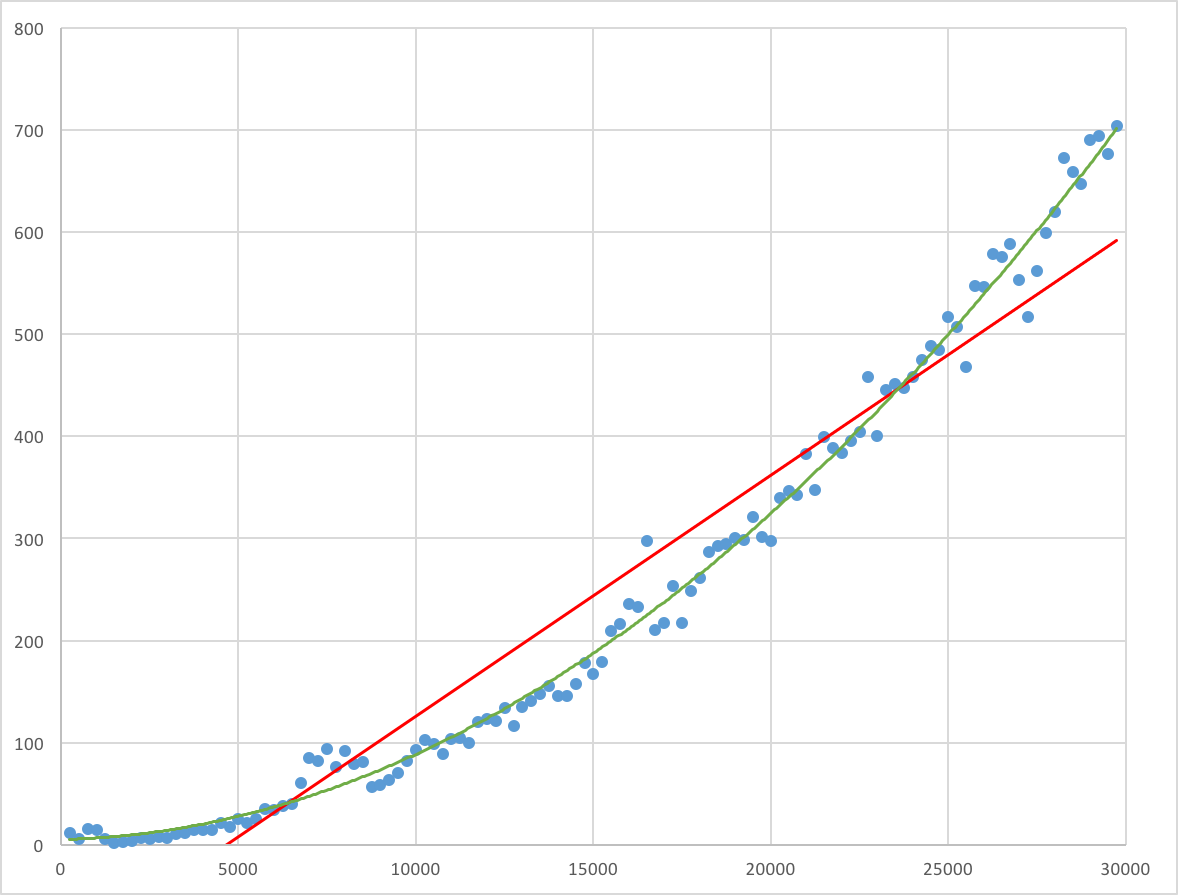
\includegraphics[width=100mm]{./img/selection_sort_linear_trendline.png}}}
	\caption{Linear regression model of selection sort runtime samples.}
	\label{fig:selection_sort_linear_trendline}
\end{figure}

The model can then be used to formulate simple predictions, $a'x + b'$ being the prediction for \textit{input descriptor} $x$. Next, we need to find a way how to determine the certainty of the prediction to be able to select the best function with given certainty using a set of these models.

\subsubsection{Confidence interval based selection from two functions}
\label{subsubsec:confidence_interval_selection}

Suppose we have the linear regression model \(h'(x) = a' x + b'\) that approximates the function $h(x) = ax + b$ constructed using \(n\) data samples \(x_i, y_i\) (in our case, \(x_i\) are the \textit{input descriptors} and \(y_i\) are the run times). If we assume that the errors $\varepsilon_i = y_i - h'(x_i)$ of our sample from the regression model values are random variables with normal distribution, we can perform some observation about the model.

Firstly, the standard errors $se(b')$ and $se(a')$ of the intercept $b'$ and the slope $a'$ can be derived from the model. In addition, the statistics $t_a = \frac{a' - a}{se(a')}$ and $t_b = \frac{b' - b}{se(b')}$ have a t-distribution with $n-2$ degrees of freedom. This means that we are able to construct confidence intervals and perform t-tests for $a$ and $b$. The default tests hypotheses have the following form:

\[H_0:\; a = a_0\]
\[H_1:\; a \neq a_0 \]

We basically test equality of $a$ (or $b$) and a fixed value $a_0$ (or $b_0$) - this test can be used to verify if the data have a specific linear relation. If we put $a_0 = 0$, we can find out whether the observations $y_i$ are constant. 

None of these tests and statistics, however, allows us to test the certainty of the prediction - we need to consider both the intercept and the slope estimation certainty, and, in addition, the distance of the $x$ we want the prediction for from the mean $\bar{x}$. The reason is that if we commit an error in the slope estimation $a'$, the corresponding error in predictions increases with the distance from $\bar{x}$. 

With these facts, a confidence interval on level $1 - \alpha$ for the mean of the actual values ($y$) for $x$ can be constructed. According to \cite{weiss_introductory_2010}, the width of the interval is the following:

%TODO: Change the text to "mean prediction interval"

\[
w_{x, \alpha} = t_{n - 2}(1-\frac{\alpha}{2}) s_e\sqrt{\frac{1}{n} + \frac{(x - \bar{x})^2}{ \sum_{i = 1}^{n} (x_i - \bar{x})^2 }}
\]

where \(\bar{x}\) is the mean of \(x_i\), $t_{n - 2}(1-\frac{\alpha}{2})$ is the $(1-\frac{\alpha}{2})$-th quantile of \textit{t-distribution} with $n-2$ degrees of freedom, and $s_e$\footnote{Standard error of the estimate} can be computed as:

\[s_e = \sqrt{\frac{SSE}{n-2}}\]

and

\[SSE = \sum_{i = 1}^{n} \varepsilon_i^2  =  \sum_{i = 1}^{n} (y_i - y_i')^2 \]

for \(y_i' = h'(x_i)\).

It now holds for any $x$ that the mean of $y = h(x)$ lies in $[a'x + b' \pm w_{x, \alpha}]$ with probability $(1-\alpha)$.

Now in the situation where we have two regression models and we want to find the best prediction of $x$, we can construct these confidence intervals for both models and:

\begin{itemize}
	\item If the intervals do not overlap, the predictions have at least a $(1 - \alpha)^2$ probability of correctly setting the order, i.e. the worse prediction actually being the worse function
	\item If the intervals overlap, there is a non-trivial chance of the predictions being mixed up by error
\end{itemize}

In the first case, we can decide that one function is significantly better and select it. In the second case, we cannot decide with given certainty.

\subsubsection{Confidence interval based selection from multiple functions}

The described method allows us to decide between two functions with given certainty. Now, when choosing among $n$ functions with regressions $h'_1, \dots, h'_n$ for given $x$, we are looking for the $k$ for which the following holds:

\begin{itemize}
	\item The confidence interval on level $(1-\alpha)$ for prediction $h'_k(x)$ does not overlap with any other of the confidence interval for prediction.
	\item $\forall j \ne k: h'_k(x) < h'_j(x)$
\end{itemize}

It can be done by constructing all the regression models and then $\forall i$ performing the comparison described in \ref{subsubsec:confidence_interval_selection} of $h_i$ with $h_j, \forall j \ne i$. If $h_i$ is better than all of the $h_j$, we can choose the corresponding function.

The strength of this decision is influenced by the fact that we perform multiple confidence interval constructions - the errors an error in any of them can influence the result of the selection, se the significance gets lower in general. If we wanted the results to be precise, we would have to perform the correction of the significance level $\alpha$. Just like in \ref{subsec:t_test_multiple}, we will leave the significance correction analysis as a potential future work.

\subsubsection{Selection algorithm}

The strategy is parametrized by the selection significance level $\alpha$ and by the secondary strategy to be used in case of decision failure.

\begin{algorithmic}[1] % The number tells where the line numbering should start
	\INPUT Historical data vectors $d_1,...,d_n$ where $d_i = [(x_{i,1}, y_{i,1}),...,(x_{i,l_i}, y_{i,l_i})]$, \textit{input descriptor} $x$
	\For{$i=1$ to $n$}
	\State $r_i \gets$ createRegression($d_i$) \Comment{Uses the least squares method}
	\EndFor
	\For{$i = 1$ to $n$}
	\State $better \gets$ true
	\For{$j = 1$ to $n$, $j \ne i$}
	\State $(k_1, l_1) \gets$ predictionInterval($r_i, x, \alpha$)
	\State $(k_2, l_2) \gets$ predictionInterval($r_j, x, \alpha)$
	\If{$(k_1, l_1)$ overlaps $(k_2, l_2)$ or $k_1 > k_2$}
	\State $better \gets$ false
	\EndIf
	\EndFor
	\If{$better$}
	\State \Return{$i$}
	\EndIf
	\EndFor
	\State \Return{useSecondaryStrategy($d_1,\dots,d_n, x$)}
\end{algorithmic}

\subsection{Window-bound linear regression}
\label{subsec:window_bound_regression}

To be able to apply the strategy described in section \ref{subsec:simple_linear_regression} on a wider variety of functions, a simple approach to lower the approximation errors can be taken. Instead of creating a regression model for the entire set of historical measurements at once, we can split it into more subsets and create different regressions for them. Figure \ref{fig:window_examples} shows ranges $5000$ to $10000$, $10000$ to $15000$ and $15000$ to $20000$ of the input sizes of the data from \ref{fig:selection_sort_linear_trendline}. As we can observe from the second and third range, the data tend to be much closer to the linear regression line. The first range shows that a less significant fluctuation in the entire set has a lot bigger impact on the model in a smaller subset.

\begin{figure}[h!]
	\captionsetup{justification=centering,margin=0.5cm}
	\centerline{\mbox{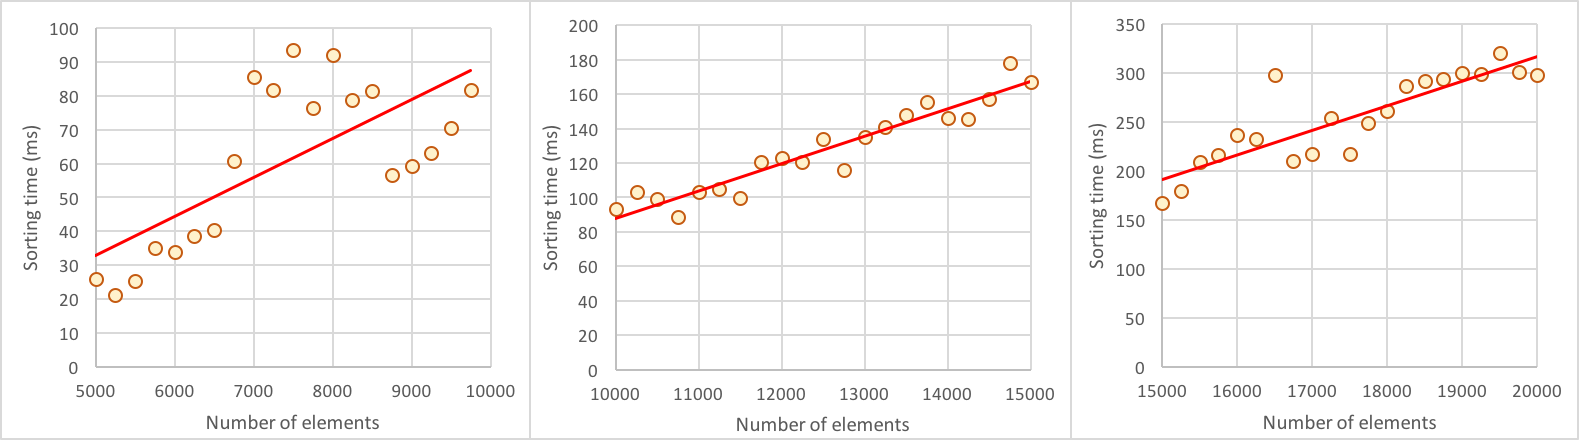
\includegraphics[width=150mm]{./img/window_examples.png}}}
	\caption{Examples of subsets of the data from figure \ref{fig:selection_sort_linear_trendline} with corresponding linear regressions.}
	\label{fig:window_examples}
\end{figure}

When selecting a function for a specific \textit{input descriptor} $x$, a window around its value of specific width $w$ can be created and the regression model built using the data from the said window. We do it by selecting only the historical samples $(x_k, y_k)$ where $\abs{x_k - x} < w$ when constructing the regression.

There are multiple ways how to decide on the window width $w$. Using a fixed number across all the functions and all the data samples would not be recommendable, as the functions can vary in their \textit{input descriptors} by orders of magnitude. The width could be derived as a fraction of the width of the whole data set: $w = \frac{max(x_i) - min(x_i)}{p}$, where $p$ would represent in how many parts we want it to be split. 

More flexible approach is to dynamically determine the $p$. Suppose we want the average window to contain $r$ records. We find out what is the average distance between two neighboring records as $d =  \frac{max(x_i) - min(x_i)}{n - 1}$ and then set the $w = r * d$. This way, the window size will always be adapted to the density of the dataset.

The window limitation might seem similar to the grouping described in \ref{subsec:grouping}, but there are two major differences. First, the windows are based on the \textit{input descriptor}, whereas the \textit{group selector} might use different features of the input. And second, the groups are deterministic and do not move with the \textit{input descriptor} and change their size based on historical data. Both these concept can be used at the same time.

\subsubsection{Selection algorithm}

The strategy is parametrized by the selection significance level $\alpha$ and by the average record count per window $avg$.

\begin{algorithmic}[1] % The number tells where the line numbering should start
	\INPUT Historical data vectors $d_1,...,d_n$ where $d_i = [(x_{i,1}, y_{i,1}),...,(x_{i,l_i}, y_{i,l_i})]$, \textit{input descriptor} $x$
	\For{$i=1$ to $n$}
	\State $dist \gets (max(x_{i,j}) - min(x_{i,j})) / (l_i-1)$
	\State $w \gets dist * avg$
	\State $d'_i \gets [(x_{i,j}, y_{i, j}); \forall j: \abs{x_{i,j} - x} \leq w/2]$
	\EndFor
	\State \Return{useLinearRegressionStrategy($d'_1,...,d'_n, x$)}
\end{algorithmic}

\subsection{Local regression}
\label{subsec:local_regression}

The approach explained in \ref{subsec:window_bound_regression} can be extended further - the locally constructed linear regression models might be used to build up a model for the entire data set. This leads to a model that is non-linear, i.e., the function that approximates the original data relation is not a linear function.

One possible regression method that behaves this way is \textit{LOESS} (Local Regression, \cite{cleveland_locally_1988,cleveland_regression_1988,cleveland_computational_1991}). It uses techniques similar to the least-square regression on local subsets of the data set, and then smooths up the resulting curve. The output is a \textit{Loess Curve}, an artificially constructed function that does not necessarily have to be expressed by a formula. This is one of the advantages of the model - the original relation between \textit{input descriptors} and the run times did not have to be expressed by a simple function in order to be captured correctly.

The \textit{LOESS} model can be used to predict the function run times. It is, however, a lot more complicated to derive the prediction confidence intervals. Therefore, only the values will be used in this selection strategy, which could lead to some wrong decisions.

There are other disadvantages of this strategy as well. First of all, the entire local regression model has to be recomputed whenever there is a new record in the dataset, the model cannot be simply updated like the \textit{simple linear regression}. Secondly, it is much more computationally complex and the model construction takes non-trivial time, so it has a negative impact on the framework overhead, especially when used with short and simple functions. The last downside of \textit{local regression} is its inability to predict further behavior past the minimum and maximum data sample.

\subsubsection{Selection algorithm}

The strategy is parametrized by the secondary strategy to be used in case of decision failure.

\begin{algorithmic}[1] % The number tells where the line numbering should start
	\INPUT Historical data vectors $d_1,...,d_n$ where $d_i = [(x_{i,1}, y_{i,1}),...,(x_{i,l_i}, y_{i,l_i})]$, \textit{input descriptor} $x$
	\For{$i=1$ to $n$}
	\State $m_i \gets$ interpolateLoess($d_i$)
	\State $p_i \gets$ predictValue($m_i, x$)
	\If{$p_i = NaN$}\Comment{The prediction can fail}
	\State\Return{useSecondaryStrategy($d_1,\dots,d_n, x$)}
	\EndIf
	\EndFor
	\State\Return{$argmin(p_i)$}
\end{algorithmic}

\subsection{Window-bound t-test}
\label{subsec:window_bound_t_test}

The mean based t-test selection strategy described in sections \ref{subsec:t_test_two} and \ref{subsec:t_test_multiple} works under the assumption that the run times of a specific function have a normal distribution, and the prediction of run time is simply the mean of all the times measured. This could be true only for the functions with constant complexity - whenever the function run time depends on the input, the samples measured have their distribution influenced by the distribution of the inputs.

\begin{figure}[h!]
	\captionsetup{justification=centering,margin=0.5cm}
	\centerline{\mbox{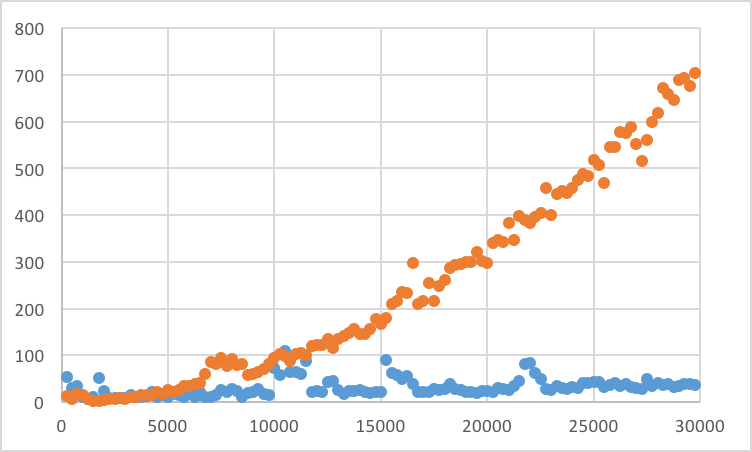
\includegraphics[width=100mm]{./img/quick_vs_selection.png}}}
	\caption{Run times of quick sort algorithm (dark dots) and selection sort algorithm (light dots) by input size.}
	\label{fig:quick_vs_selection}
\end{figure}

\begin{figure}[h!]
	\captionsetup{justification=centering,margin=0.5cm}
	\centerline{\mbox{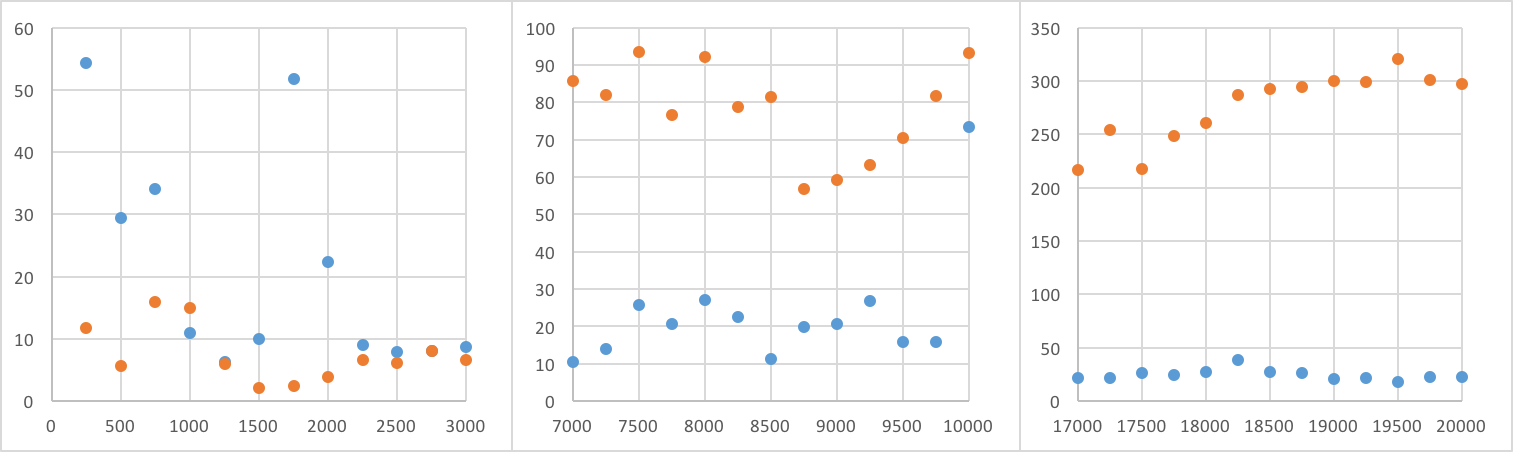
\includegraphics[width=150mm]{./img/window_t_test_examples.png}}}
	\caption{Examples of subsets of the data from figure \ref{fig:quick_vs_selection}}
	\label{fig:window_t_test_examples}
\end{figure}

If we wanted to use the t-test strategy on the functions with non-constant complexity, the same approach as with the \textit{simple linear regression} can be taken. Instead of assuming that the relation in the small window is linear, we want it to be constant and normally distributed. We can then predict the run time using the mean of the measurements from within a very small range of \textit{input descriptor} values. Consequently, it is extremely important to keep the window size as small as possible, so that these assumptions held at least approximately. The t-test significance levels and strengths will be approximate as well, but our goal is to get reasonable selection behavior, we do not need to be precise.

Figure \ref{fig:quick_vs_selection} shows the run times measured for the quick sort and selection sort algorithms on random arrays of sizes between $0$ and $30000$. Obviously, there is a relation to the input size, so the simple t-test should not be applied in this case. In figure \ref{fig:window_t_test_examples}, there are the same data in three different windows - $0$ to $3000$, $7000$ to $10000$ and $17000$ to $20000$. As we can see, in a window of this size, the run times are almost constant and the random fluctuations are more significant than the actual relation to the input size. We can apply the t-test as described in sections \ref{subsec:t_test_two} and \ref{subsec:t_test_multiple} to these windows and consider the result to be relevant enough with respect to the input.

The window sizes can be determined in a similar way as in section \ref{subsec:window_bound_regression}. If we reduce it to a constant 0, we will get a technique in which only the results for inputs with the same descriptor are tested. When there are none, we refuse to select and wait until data are gathered. This might be useful in cases where we know that the function will be called repeatedly on a limited set of input variants, and basically rules out the prediction factor, as we need to have actual observation for each input before making any conclusions. Similar approach is taken in \cite{bulej_performance_2012}. The same goal, however, can be achieved more efficiently using the grouping mechanism (see \ref{subsec:grouping}).

\subsubsection{Selection algorithm}

The strategy is parametrized by the selection significance level $\alpha$ and by the average record count per window $avg$.

\begin{algorithmic}[1] % The number tells where the line numbering should start
	\INPUT Historical data vectors $d_1,...,d_n$ where $d_i = [(x_{i,1}, y_{i,1}),...,(x_{i,l_i}, y_{i,l_i})]$, \textit{input descriptor} $x$
	\For{$i=1$ to $n$}
	\State $dist \gets (max(x_{i,j}) - min(x_{i,j})) / (l_i-1)$
	\State $w \gets dist * avg$
	\State $d'_i \gets [(x_{i,j}, y_{i, j}); \forall j: \abs{x_{i,j} - x} \leq w/2]$
	\EndFor
	\State \Return{useTTestStrategy($d'_1,...,d'_n$)}
\end{algorithmic}

\subsection{Whitebox model construction}

The methods that were described so far are examples of the blackbox techniques - they do not analyze the function itself, the models are based only on the relation of the run times and the \textit{input descriptors}. 

The techniques used in the research projects focused on formulating accurate predictions about program run times (like \cite{goldsmith_measuring_2007,chun_mantis:_2010,huang_predicting_2010}) often build the model using more detailed information about every run. These extra data can be obtained by examining and instrumenting the function code. Key structures (loops, branches, method invocation, ...) can be identified and execution counts can be tracked. Then, a model that captures the relation between the input features, the described structure execution counts and the run time can be constructed. This added dimension might lead to more accurate model and therefore better predictions.

%TODO: Add reference / bibliography
In \cite{chun_mantis:_2010}, a Mantis framework for high accuracy program performance prediction was implemented. The basic principles are similar to the approach described above. It was tested on a series of data gathered from runs of the ImageJ application, and compared with a blackbox prediction model based on interpolating a polynomial of degree three. The prediction error of the whitebox approach was 5.5\%, the blackbox approach error rate reached more than 35\%.
%TODO: Add results?

This approach has, however, a few problems concerning the intended use cases of our framework. The model will not improve the predictions if the majority of the execution time is spent waiting on an I/O operation. Specifically, it will not help with any of the cases where we are selecting a database query, remote server to connect to, etc. In addition, it would require the method code to be instrumented at runtime, which would lead, together with the model construction, to a significant overhead.

For these reasons and because of the complexity, the whitebox model was not implemented in the framework, but it represents a potential future work that could be done on the topic.

\section{Strategy comparison}
\label{sec:strategy_comparison}

In general, the input based strategies do not handle well more historical results for the same \textit{input descriptor}, and are impossible to use when there is none specified. The following rules should be used to decide between input based and mean based strategies:

\begin{itemize}
	\item \textbf{Dependency on the input} \\
	If the function does not have any input, or the input does not affect the expected run time (the complexity is constant), mean based strategies should be used.
	\item \textbf{Expected input values} \\
	If the function is expected to be invoked with a discrete and very limited set of inputs, mean based strategy is preferred. On the other hand, if the function will be called repeatedly with randomly distributed inputs, the input based strategies are a better choice.
\end{itemize}

Considering these facts, the framework will contain both an input based and a mean based strategy, and will automatically use the input based one if the user specified an \textit{input descriptor}, and the mean based one otherwise. The user will be able to override this choice if he wants.

The actual strategies used should be easily replaceable, but some have to be chosen as default for the common uses. Therefore, a practical comparison of the selection success rate and overheads of the strategies that were described and implemented follows.

\subsection{Input based strategies success rates}
\label{subsec:input_based_strategies_success}

To compare the efficiency of the selection strategies, we will perform two tests. The first one will be based on an artificial function with linear complexity defined by the following lambda expression:

\lstset{style=Scala}
\begin{lstlisting}
i => {
  val j = (i * k).toInt
  var acc = 0
  Seq.range(0, j).foreach(l => {
    acc = acc + (l * Random.nextInt(1000))
  })
  acc
}
\end{lstlisting}

Where \inlinecode{i} is the input of the function and \inlinecode{k} is a constant factor which can be used to slow the function down.

Analogically, we will define a quadratic function (using a similar lambda, only with second line replaced by \inlinecode{val j = (i * i * k).toInt}).

Now, the test will be based on combining two instances of the same function\footnote{Note that the actual implementation requires either using two different lambdas, or using custom identifiers, more on that topic in section \ref{subsec:function_identifiers}}, one with $k=1$ and the other with some $k>1$, perform a series of runs and track how many times will the selection strategy choose the worse one (i.e. the $k>1$ one).

For each test, we will generate 100 sequences, each one containing 200 integers between 100000 and 500000 in case of the linear function, or 100 and 500 for the quadratic function. One sequence will represent one test run - the measurement history will be flushed and the function will be invoked on the members of the sequence one by one. The strategies are set in the way that the first 60 runs will use a round-robin selection to gather 30 data samples for each function before starting the actual selection. It means that the strategy should perform 140 selections for each test run. We are going to count how many times the worse function is selected. The baseline solution in this case would be to keep using the round-robin technique, which would lead to the worse function being selected 50\% of the time, 70 times out of 140.

Now, we will use the following values for $k$: 4, 2, 1.5, 1.2, 1.1, 1.01, and the following selectors:
\begin{itemize}
	\item Window-bound t-test (WBTT) with $\alpha$ set to 0.05 and 0.25
	\item Linear regression (LR) with $\alpha$ set to 0.05 and 0.25
	\item Window-bound linear regression (WBLR) with $\alpha$ set to 0.05 and 0.25
	\item Local regression (LOESS)
\end{itemize}

For each combination, all 100 test runs were performed and an average percentage of the worse function selection was computed, the results for the linear function can be seen in table \ref{tab:strategy_comparison} and for the quadratic function in table \ref{tab:strategy_comparison_quadratic}. A surprising fact might be the overall better results for the non-linear case, which should be more difficult to model. The reason for this fact is that there is a dramatically lower range of inputs (100 to 500 instead of 100000 to 500000) in order to keep the test run time realistic. In addition, the run time differences between individual inputs grows much faster, so the error factor involved does less damage to the model. In general, it seems that functions with faster-growing complexities get more precise predictions.


\begin{table}[h!]
	\captionsetup{justification=centering,margin=0.5cm}
	\centering
	\bgroup
	\def\arraystretch{1.5}%
	\begin{tabular}{|l|r|r|r|r|r|r|r|}
		\hline
		\textbf{}      & \multicolumn{1}{c|}{\textbf{\begin{tabular}[c]{@{}c@{}}WBTT\\ (0.05)\end{tabular}}} & \multicolumn{1}{c|}{\textbf{\begin{tabular}[c]{@{}c@{}}LR\\ (0.05)\end{tabular}}} & \multicolumn{1}{c|}{\textbf{\begin{tabular}[c]{@{}c@{}}WBLR\\ (0.05)\end{tabular}}} & \multicolumn{1}{c|}{\textbf{\begin{tabular}[c]{@{}c@{}}WBTT\\ (0.25)\end{tabular}}} & \multicolumn{1}{c|}{\textbf{\begin{tabular}[c]{@{}c@{}}LR\\ (0.25)\end{tabular}}} & \multicolumn{1}{c|}{\textbf{\begin{tabular}[c]{@{}c@{}}WBLR\\ (0.25)\end{tabular}}} & \multicolumn{1}{c|}{\textbf{LOESS}} \\ \hline
		\textbf{1.01x} & 52.4\%                                                                              & 49.6\%                                                                            & 51.5\%                                                                              & 47.1\%                                                                              & 49.6\%                                                                            & 50.1\%                                                                              & 43.6\%                              \\ \hline
		\textbf{1.1x}  & 49.4\%                                                                              & 48.5\%                                                                            & 37.2\%                                                                              & 33.7\%                                                                              & 44.6\%                                                                            & 33.5\%                                                                              & 6.2\%                               \\ \hline
		\textbf{1.2x}  & 40.1\%                                                                              & 46.0\%                                                                            & 29.0\%                                                                              & 26.3\%                                                                              & 41.6\%                                                                            & 27.8\%                                                                              & 3.5\%                               \\ \hline
		\textbf{1.5x}  & 30.2\%                                                                              & 38.9\%                                                                            & 13.9\%                                                                              & 13.7\%                                                                              & 25.6\%                                                                            & 9.9\%                                                                               & 2.9\%                               \\ \hline
		\textbf{2x}    & 17.6\%                                                                              & 25.4\%                                                                            & 7.8\%                                                                               & 4.3\%                                                                               & 14.4\%                                                                            & 4.7\%                                                                               & 2.4\%                               \\ \hline
		\textbf{4x}    & 2.9\%                                                                               & 15.7\%                                                                            & 5.0\%                                                                               & 0.1\%                                                                               & 9.7\%                                                                             & 2.7\%                                                                               & 2.5\%                               \\ \hline
	\end{tabular}
	\egroup
	\caption{Percentage of times the strategy selected the worse one out of two linear functions (average from 100 test runs, each containing 140 selections).}
	\label{tab:strategy_comparison}
\end{table}

\begin{table}[h!]
	\captionsetup{justification=centering,margin=0.5cm}
	\centering
	\bgroup
	\def\arraystretch{1.5}%
	\begin{tabular}{|l|r|r|r|r|r|r|r|}
		\hline
		\multicolumn{1}{|c|}{\textbf{}} & \multicolumn{1}{c|}{\textbf{\begin{tabular}[c]{@{}c@{}}WBTT\\ (0.05)\end{tabular}}} & \multicolumn{1}{c|}{\textbf{\begin{tabular}[c]{@{}c@{}}LR\\ (0.05)\end{tabular}}} & \multicolumn{1}{c|}{\textbf{\begin{tabular}[c]{@{}c@{}}WBLR\\ (0.05)\end{tabular}}} & \multicolumn{1}{c|}{\textbf{\begin{tabular}[c]{@{}c@{}}WBTT\\ (0.25)\end{tabular}}} & \multicolumn{1}{c|}{\textbf{\begin{tabular}[c]{@{}c@{}}LR\\ (0.25)\end{tabular}}} & \multicolumn{1}{c|}{\textbf{\begin{tabular}[c]{@{}c@{}}WBLR\\ (0.25)\end{tabular}}} & \multicolumn{1}{c|}{\textbf{LOESS}} \\ \hline
		\textbf{1.01x}                  & 52.3\%                                                                              & 49.4\%                                                                            & 44.6\%                                                                              & 50.5\%                                                                              & 50.3\%                                                                            & 49.5\%                                                                              & 44.6\%                              \\ \hline
		\textbf{1.1x}                   & 44.9\%                                                                              & 43.1\%                                                                            & 28.9\%                                                                              & 33.3\%                                                                              & 37.8\%                                                                            & 26.2\%                                                                              & 7.4\%                               \\ \hline
		\textbf{1.2x}                   & 38.2\%                                                                              & 38.1\%                                                                            & 16.3\%                                                                              & 17.8\%                                                                              & 31.2\%                                                                            & 15.7\%                                                                              & 4.0\%                               \\ \hline
		\textbf{1.5x}                   & 16.6\%                                                                              & 28.7\%                                                                            & 8.4\%                                                                               & 7.9\%                                                                               & 18.5\%                                                                            & 6.4\%                                                                               & 2.5\%                               \\ \hline
		\textbf{2x}                     & 8.8\%                                                                               & 20.0\%                                                                            & 4.1\%                                                                               & 2.7\%                                                                               & 13.4\%                                                                            & 2.4\%                                                                               & 2.3\%                               \\ \hline
		\textbf{4x}                     & 3.5\%                                                                               & 19.6\%                                                                            & 3.0\%                                                                               & 0.1\%                                                                               & 14.6\%                                                                            & 1.5\%                                                                               & 2.3\%                               \\ \hline
	\end{tabular}
	\egroup
	\caption{Percentage of times the strategy selected the worse one out of two quadratic functions (average from 100 test runs, each containing 140 selections).}
	\label{tab:strategy_comparison_quadratic}
\end{table}

As to the individual strategies, it might be unexpected that the linear regression has quite poor results, even in the case where the original function complexities were linear. Almost $16\%$ of selections of a function that is four times slower in the $\alpha = 0.05$ case. This is caused by the fact that eventual measurements with extreme deviations influence the whole model, not just a local part of it, which might lead to an eventual series of wrong decisions. Therefore, linear regression strategy is not recommended to be used in general.

On the other hand, the absolute winner is the local regression, which is able to maintain extremely low error rates ($6.2\%$ for the linear functions, $7.4\%$ for the quadratic functions) for the second-minimal case $k=1.1$, and push it even lower with growing $k$. Neither one of the other strategies got below $15\%$ not only for $k=1.1$, but even for $k=1.2$.

The window-bound strategies are somewhere in the middle - they perform very well for higher $k$ ($2, 4$), which is the main concern, and reasonably for the other sizes. The main difference between them being that the window-bound linear regression improves steadily with growing $k$, whereas the window-bound t-test reaches better results for the largest $k=4$, but improves dramatically at the end and has worse results for lower $k$.

We can see that in all the cases, lowering the selection significance (by increasing the $\alpha$) can lead to slightly better results overall, especially for larger values of $k$. The success of local regression, which does not employ certainty in the decision making process, supports this observation. It seems that the assumption of selection errors having a bad influence on the model and leading to chains of bad decisions was not confirmed by this test. It might be, however, different for real-life scenarios with more variable run times, environment changes, etc., and we should keep that in mind and be careful when lowering the $\alpha$ for better selection results.

\subsection{Mean based strategies success rates}

Similarly to the input based strategies, we are going to perform a selection success rate test for the mean based strategies. As we need only a function with fixed non-trivial execution time with a possibility to slow it down a little, we are going to reuse the linear function from section \ref{subsec:input_based_strategies_success}, fixing its input to 200000. Again, we are going to combine an instance of the non-slowed function with the instances of function slowed by a factor $k$. 

The values 2, 1.5, 1.2, 1.1, 1.01 will be used for $k$, along with the following selectors:
\begin{itemize}
	\item T-test (TT) with $\alpha$ set to 0.05 and 0.25
	\item U-test (UT) with $\alpha$ set to 0.05 and 0.25
\end{itemize}

For each combination of $k$ and a selector, 100 test runs will be performed, each one consisting of invoking the described combined function 200 times and removing all the history records afterwards.

The results can be seen in table \ref{tab:strategy_comparison_mean_based}. It might seem obvious that the u-tests deliver better results, and again, lowering the $\alpha$ improves the result as well. In order to get more insight into the results, we should take into account another factor - the number of test runs, where the overall success rate was worse than the baseline success rate, i.e. the $50\%$ of the round-robin selection. This is shown in the table \ref{tab:strategy_comparison_mean_based_worse_runs}.

\begin{table}[h!]
	\captionsetup{justification=centering,margin=0.5cm}
	\centering
	\bgroup
	\def\arraystretch{1.5}%
	\begin{tabular}{|l|r|r|r|r|}
		\hline
		& \multicolumn{1}{c|}{\textbf{\begin{tabular}[c]{@{}c@{}}TT\\ (0.05)\end{tabular}}} & \multicolumn{1}{c|}{\textbf{\begin{tabular}[c]{@{}c@{}}UT\\ (0.05)\end{tabular}}} & \multicolumn{1}{c|}{\textbf{\begin{tabular}[c]{@{}c@{}}TT\\ (0.25)\end{tabular}}} & \multicolumn{1}{c|}{\textbf{\begin{tabular}[c]{@{}c@{}}UT\\ (0.25)\end{tabular}}} \\ \hline
		\textbf{1.01x} & 49.8\%                                                                            & 49.5\%                                                                            & 49.8\%                                                                            & 47.1\%                                                                            \\ \hline
		\textbf{1.1x}  & 46.6\%                                                                            & 27.0\%                                                                            & 39.1\%                                                                            & 25.5\%                                                                            \\ \hline
		\textbf{1.2x}  & 42.2\%                                                                            & 18.5\%                                                                            & 25.6\%                                                                            & 14.3\%                                                                            \\ \hline
		\textbf{1.5x}  & 11.6\%                                                                            & 0.0\%                                                                             & 2.6\%                                                                             & 0.2\%                                                                             \\ \hline
		\textbf{2x}    & 1.9\%                                                                             & 0.0\%                                                                             & 0.0\%                                                                             & 0.0\%                                                                             \\ \hline
	\end{tabular}
\egroup
\caption{Percentage of times the strategy selected the worse one out of two constant functions (average from 100 test runs, each containing 140 selections).}
\label{tab:strategy_comparison_mean_based}
\end{table}

\begin{table}[h!]
	\captionsetup{justification=centering,margin=0.5cm}
	\centering
	\bgroup
	\def\arraystretch{1.5}%
	\begin{tabular}{|l|r|r|r|r|}
		\hline
		& \multicolumn{1}{c|}{\textbf{\begin{tabular}[c]{@{}c@{}}TT\\ (0.05)\end{tabular}}} & \multicolumn{1}{c|}{\textbf{\begin{tabular}[c]{@{}c@{}}UT\\ (0.05)\end{tabular}}} & \multicolumn{1}{c|}{\textbf{\begin{tabular}[c]{@{}c@{}}TT\\ (0.25)\end{tabular}}} & \multicolumn{1}{c|}{\textbf{\begin{tabular}[c]{@{}c@{}}UT\\ (0.25)\end{tabular}}} \\ \hline
		\textbf{1.01x} & 0                                                                                 & 1                                                                                 & 19                                                                                & 7                                                                                 \\ \hline
		\textbf{1.1x}  & 0                                                                                 & 15                                                                                & 5                                                                                 & 20                                                                                \\ \hline
		\textbf{1.2x}  & 0                                                                                 & 15                                                                                & 4                                                                                 & 13                                                                                \\ \hline
		\textbf{1.5x}  & 0                                                                                 & 0                                                                                 & 0                                                                                 & 0                                                                                 \\ \hline
		\textbf{2x}    & 0                                                                                 & 0                                                                                 & 0                                                                                 & 0                                                                                 \\ \hline
	\end{tabular}
\egroup
\caption{The number of test runs (out of 100) where the strategy had a success rate worse than 50\%.}
\label{tab:strategy_comparison_mean_based_worse_runs}
\end{table}

It looks like the t-test is more conservative, it refuses to make the decision more often, which leads to switching the functions in the round-robin fashion. On the other hand, the u-test risks more, which leads to better results overall, but there are some runs that are very bad - for $k=1.2$, $15$ runs out of $100$ were worse than $50\%$, and $10$ out of these $15$ runs had a $0\%$ success rate, which means that the model selected the worse function every time.

The conclusion from the observations is that employing u-test (or increasing the $\alpha$) increases the expected success rate in a common case, but brings a non-trivial risk of constructing a wrong model which leads to a sequence of errors that might last very long.

\subsection{Strategy performance}
\label{subsec:strategy_perf}

When deciding for one of the strategies, there is another concern that we should keep in mind. The strategies tend to be quite complex and their execution time might become non-trivial. As they need to process the entire run history of each of the functions, their selection times increase over time, as more historical measurements are collected.

For some of the strategies, it is possible to compute and cache the statistical data in advance, at the moment of storing newly measured data, allowing them to avoid processing all the records again during the selection. From our strategy list, this is possible to be done for the linear regression and the t-tests. Unfortunately, neither the window-bound strategies, nor the local regression support this approach.

To compare the practical overheads, we ran the selection using each of the strategies 20000 times in a row (while evaluating the runs and adding new data in the process) for the task of deciding between quick sort and selection sort algorithm on sequences of 0 to 2000 numbers. The window-bound strategies had the window size calculated to contain 25 records in average. The resulting averages of selection strategy run times are in table \ref{tab:strategy_execution_comparison}.

\begin{table}[h!]
	\captionsetup{justification=centering,margin=0.5cm}
	\centering
	\bgroup
	\def\arraystretch{1.5}%
	\begin{tabular}{|l|r|r|}
		\hline
		\textbf{}                  & \multicolumn{1}{l|}{\textbf{Not cached}} & \multicolumn{1}{l|}{\textbf{Cached}} \\ \hline
		\textbf{Linear regression} & 1.68                                     & 0.15                                 \\ \hline
		\textbf{Window-bound LR}   & 0.91                                     & -                                  \\ \hline
		\textbf{Window-bound TT}   & 0.72                                     & -                                  \\ \hline
		\textbf{LOESS}             & 57.47                                    & -                                  \\ \hline
		\textbf{T-test}            & 1.32                                     & 0.10                                 \\ \hline
		\textbf{U-test}            & 5.91                                     & -                                  \\ \hline
	\end{tabular}
\egroup
\caption{Average strategy selection time (in ms) in a sequence of 20000 consecutive selections.}
\label{tab:strategy_execution_comparison}
\end{table}


The results are showing that local regression has extremely high run times that can grow above 50 milliseconds for situations with larger number of historical observations. An overhead of this size on every selection would be too high for most common usages, so the local regression strategy, even though it has the best success rate, should be used with extreme caution and only in cases where it is clear that overhead this high cannot damage the system performance. 

As for the remaining strategies, it seems that caching speeds up the selection a little more than 10 times for this number of runs. The window-bound strategies cannot be improved by the caching (as the relevant statistics are different for every window), but they have the lowest execution time of all the strategies without cache, and therefore are very usable for the input based case. Regarding the mean based strategies, the t-test is almost 5 times faster than the u-test in the non-cached version, and more than 50 times faster when using the cache, so it is clearly a better choice if performance is the main concern.

\section{Invocation policies}
\label{sec:policies}

The selection process and all the strategies described in sections \ref{sec:mean_based_strategies} and \ref{sec:input_based_strategies} are quite complex and have non-trivial overhead, especially after collecting a large amount of historical data, as discussed in section \ref{subsec:strategy_perf}. In a common scenario where we expect the system to come to a decision about the best function (either overall, or separately for every group), it would be suitable if we could stop the selection process at a certain point and keep using only the most favored function with no extra overhead. Or, to use it most of the time, with only occasional attempts at the selection in order to detect possible changes in the system (response times, I/O operation duration, etc.).

Similarly, it might be desirable to control the overhead time spent on the selection, or, in general, on invoking the functions using selection (which might lead to a bad decision), either per a specific time period, or with respect to a specific action of the system (user request, processing unit, etc.). All of these decisions should be taken at a higher level than the run time history analysis performed by the selection strategies.  

\textit{Invocation policies} are a concept that tries to address these cases, with the main purpose of lowering its invocation overhead. Every combined function has an \textit{invocation policy} associated with it. In the function selection chain, the policy gets evaluated right after invoking the combined function and is supposed to quickly decide how to proceed with the invocation. There might be scenarios where a faster ways could be taken without even using any of the strategies and analyzing the historical data.

The possible results of the policy evaluation are the following:

\begin{itemize}
	\item \textbf{SelectNew} - Select function using the selection strategy, executing the chain described in section \ref{sec:selection_and_invocation_process}
	\item \textbf{GatherData} - Gather more data for the least-executed function (function selection is skipped, but the run time is measured and the data are stored to the history)
	\item \textbf{UseLast} - Use the function selected last time (without measuring run time and storing it to the history)
	\item \textbf{UseMost} - Use the most selected function (without measuring run time and storing it to the history)
\end{itemize}

We can notice that these results require only the basic statistical data about previous selection processes. This is the key idea of the policies - the decision and the execution should depend only on such a simple statistics.

The policy evaluation process also replaces the current policy with a new one. This technically creates a state machine - the state of the function is represented by the active policy, and whenever the function is invoked, a result is produced and new policy becomes active. This corresponds to producing output and moving to a new state in a state machine.

The advantage of the policy system over a regular state machine is its extensibility and reusability - there are no rules directly in the state machine (i.e. here in the combined function). All the logic of deciding on the result and the next policy is in the policy node itself. So the entire behavior of the state machine is defined by the initial policy, which should be specified by the user upon creating the combined function. As a result, reusable policies that are parametrized can be used in various chains of policies, smaller chains can be put together, etc.
%TODO: Reference to the API

\subsection{Statistical data}
\label{subsec:statistical_data}

The only input that the policy receives when making decision is a statistical summary of previous selection results of the combined function. The process itself is supposed to be fast and reflect just the trends in the selection, not to replace the whole selection strategy decision making as described in sections \ref{sec:mean_based_strategies} and \ref{sec:input_based_strategies}, so the statistical data do not contain the entire run history of all the functions involved.

\begin{figure}[h!]
	\captionsetup{justification=centering,margin=0.5cm}
	\centerline{\mbox{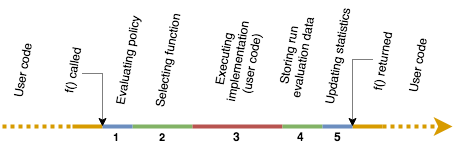
\includegraphics[width=100mm]{./img/run_schema.png}}}
	\caption{Process of combined function invocation.}
	\label{fig:run_schema}
\end{figure}

The policies are a suitable tool to limit the potential damage of the selection process to the system. For this, it is necessary to observe and to store various times connected with the selection and execution. Figure \ref{fig:run_schema} shows the whole process with policy being evaluated with the \textbf{SelectNew} result, split into individual parts. Upon every invocation, the following is tracked:

\begin{itemize}
	\item Selection and run history storage time (2 and 4)
	\item Function execution time (3)
	\item Total time spent on the \textbf{SelectNew} result (2, 3 and 4)
	\item Total time spent on the \textbf{GatherData} result (3 and 4, 2 is skipped in such a case)
\end{itemize}

Sums of these times are kept in every combined function. The policy can work with these numbers and analyze the changes that happen to them over time. In addition, the number of times each function was selected, the total number of times we received the \textbf{SelectNew} and \textbf{GatherData} result and the total number of times the combined function was invoked have to be tracked. 

In general the policy has the following data available to decide:

\begin{itemize}
	\item Total run count of the combined function
	\item Total number of times each function was selected
	\item Total number of times of gathering new data (\textbf{GatherData} result)
	\item Total time spent on function execution (after \textbf{SelectNew} result)
	\item Total time spent on selection and storage overhead (after \textbf{SelectNew} result)
	\item Total time spent on processing the \textbf{SelectNew} result
	\item Total time spent on processing the \textbf{GatherData} result
	\item Number of times the last selected function was selected in a row (the \textit{function streak})
\end{itemize}

\subsection{Implemented policies}

As mentioned earlier, policies are designed to be reusable as building-blocks. The immutable policy itself is the only holder of the state and change of state can be performed only by transitioning to a different policy. Its functionality and very simple decision-making process can be visualized using a transition diagram, which shows the policy itself as a dark (red) square with solid border, all the other policies as a lighter squares with either solid or dashed border (determines if the policy is an argument or not), and arrows as state transitions. The transitions might be conditional, in such a case, the condition splits the arrow into two. The transition can produce a result which is shown next to the transition arrow. If a result is produced, the policy makes a decision and next policy will be evaluated during the following invocation. If a result isn't produced, the policy just delegates the decision to the next policy which is evaluated immediately. The chain of evaluation stops when first result is produced.

The transition conditions use policy parameters, which are passed to a policy in the constructor, and the current statistical data explained in section \ref{subsec:statistical_data}. It can also use static fields and methods that it has access to. The parameters of the top-level (starting) policy are passed in by the user creating it, the parameters of the other policies in the chain are fixed when the policies are created, usually during the decision of the top-level policy, which typically builds the entire policy chain (that can be cyclic and lead back to it).

The transition diagrams and short descriptions of some policies will follow.

\subsubsection{Building blocks}

\begin{figure}[h!]
	\captionsetup{justification=centering,margin=0.5cm}
	\centerline{\mbox{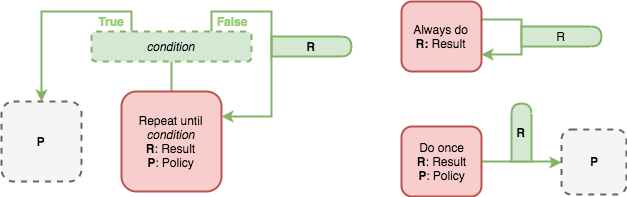
\includegraphics[width=130mm]{./img/helper_policies.png}}}
	\caption{Transition diagram of the basic building-block policies.}
	\label{fig:helper_policies}
\end{figure}

Figure \ref{fig:helper_policies} shows the main policies that serve as a building-blocks. The most important is the \textbf{Repeat until condition} policy, parametrized by a \textit{condition}, result \textit{R}, which it keeps producing until the \textit{condition} becomes true, and the policy \textit{P}, which it makes transition to at that moment. The \textbf{Always do} policy represents an infinite loop producing the same result \textit{R} every time, and the \textbf{Do once} policy produces the result \textit{R} once and immediately makes transition to the policy \textit{P}.

\begin{figure}[h!]
	\captionsetup{justification=centering,margin=0.5cm}
	\centerline{\mbox{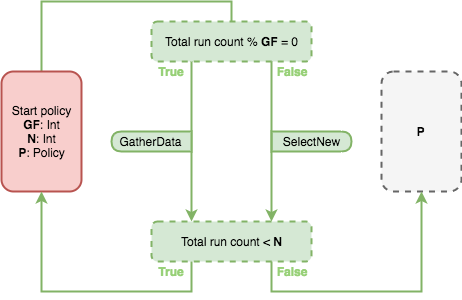
\includegraphics[width=80mm]{./img/start_policy.png}}}
	\caption{Transition diagram of the \textbf{Start policy}.}
	\label{fig:start_policy}
\end{figure}

Figure \ref{fig:start_policy} represents the \textbf{Start policy}, which accepts the gather frequency \textit{GF}, number of invocation times \textit{N} before moving to a next policy \textit{P}. It is a little more complicated and specialized version of the \textbf{Repeat until} policy - it keeps producing the \textbf{SelectNew} result, and every \textit{GF}-th invocation, it produces the \textbf{GatherData} result. It might be useful at the beginning, when it is necessary to gather data for all of the functions and perform some selections so that the following policies had statistical data to base their decision on.

\subsubsection{Stop selecting when decided}

\begin{figure}[h!]
	\captionsetup{justification=centering,margin=0.5cm}
	\centerline{\mbox{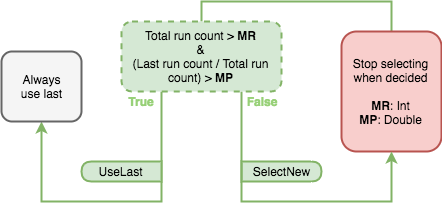
\includegraphics[width=90mm]{./img/stop_selecting_when_decided.png}}}
	\caption{Transition diagram of the \textbf{Stop selecting  when decided} policy.}
	\label{fig:stop_selecting_when_decided}
\end{figure}

In order to limit the overhead, it might be useful to completely stop selecting when we are sure that one of the functions gets selected a lot more often. The \textbf{Stop selecting when decided} policy shown in figure \ref{fig:stop_selecting_when_decided} keeps selecting new function until both the total number of invocations exceeds minimum run count \textit{MR} and the ratio of the number of times that the last selected function was selected and the total number of invocations exceeds the minimum percentage \textit{MP}. After that, it will keep using the last function forever. 

The advantage of falling back to the infinite \textbf{Always use last} policy is its basically zero overhead - no condition is evaluated in the decision process. So this policy is useful for the fast functions where keeping low overhead for the long-term is critical. It cannot, however, undo a wrong decision, reflect a change in conditions, or anything else.

\subsubsection{Pause selection after streak}

\begin{figure}[h!]
	\captionsetup{justification=centering,margin=0.5cm}
	\centerline{\mbox{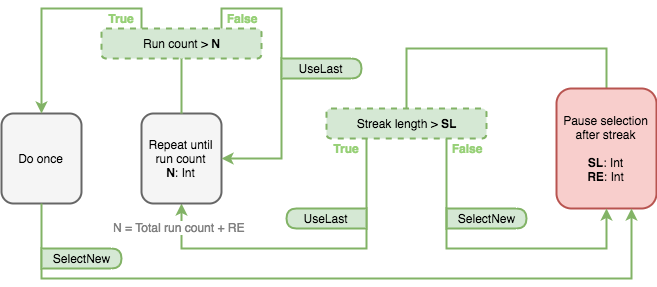
\includegraphics[width=110mm]{./img/pause_selection_after_streak.png}}}
	\caption{Transition diagram of the \textbf{Pause selection after streak} policy.}
	\label{fig:pause_selection_after_streak}
\end{figure}

To lower the number of selections, an approach based on the streak lengths can be used as well. It is implemented by the \textbf{Pause selection after streak} policy in figure \ref{fig:pause_selection_after_streak}. Its functionality is defined by the \textit{SL} (streak length) and \textit{RE} (retry every) arguments. Whenever one function is selected \textit{SL} times in a row, the selection process stops and the \textbf{UseLast} result is being produced. Once every \textit{RE} times, a new selection attempt is done, looping back to the original policy. If the same function is selected once again, the streak gets longer by one and the selection process stops again. If, however, a different function is selected this time, the streak becomes zero and we start selecting again.

The described behavior is the preferred way of limiting the selection overhead. By setting the streak length to a reasonable number (e.g. between 10 and 100, based on the data, situation, etc.), we can assure that if one function is significantly better than the others, it will be used without the need to select it. The retry that happens every once in a while makes sure that eventual wrong decision will be detected and will reset the system back to the beginning.

\subsubsection{Limited overhead, gather time and selection time}

\begin{figure}[h!]
	\captionsetup{justification=centering,margin=0.5cm}
	\centerline{\mbox{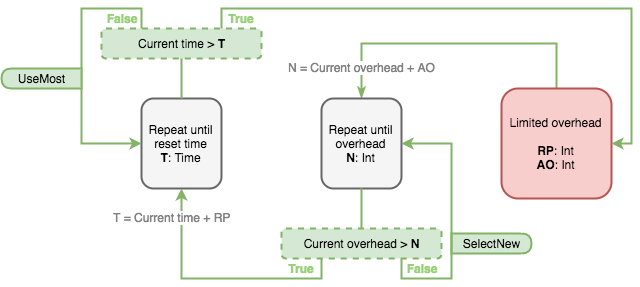
\includegraphics[width=110mm]{./img/limited_overhead.png}}}
	\caption{Transition diagram of the \textbf{Limited overhead} policy.}
	\label{fig:limited_overhead}
\end{figure}

Policies can be used to limit the framework involvement per a real-time period, so that the selection overhead or the time spent on gathering data does not damage the system more than a specified limit. The \textbf{Limited overhead} policy in figure \ref{fig:limited_overhead} limits only the selection overhead time to \textit{AO} (allowed overhead) every \textit{RP} (reset period). After depleting the allowed time, it cannot select anymore and keeps using the most selected function until the end of the period.

\begin{figure}[h!]
	\captionsetup{justification=centering,margin=0.5cm}
	\centerline{\mbox{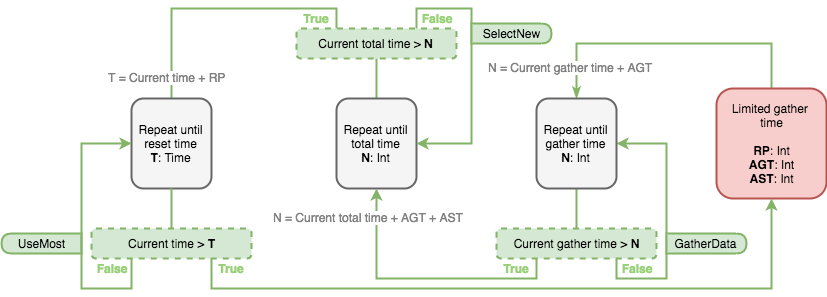
\includegraphics[width=110mm]{./img/limited_gather_time.png}}}
	\caption{Transition diagram of the \textbf{Limited gather time} policy.}
	\label{fig:limited_gather_time}
\end{figure}

In exactly the same way, the time spent on executing the function for the result \textbf{GatherData} and the whole process of selection and execution for the \textbf{SelectNew} result can be limited. The figure \ref{fig:limited_gather_time} demonstrates the \textbf{Limited gather time} policy, which keeps producing \textbf{GatherData} until total gather time reaches \textit{AGT} (allowed gather time), after that, it continues with the \textbf{SelectNew} result until total selection time reaches \textit{AST} (allowed selection time). A loop producing \textbf{UseMost} follows, for the rest of the real-time period specified by \textit{RP} (reset period).

This policy gives us control over the time spent on selecting results in real-time. If we get a lot of requests at the same time, receive a large batch of data to process or for any reason need to momentarily increase the throughput of the system, the time or overhead limits get depleted very quickly and the \textbf{UseMost} fallback result means reasonably good performance with a minimum overhead.

\subsection{Policy builder}

As we could see from the policy examples, most of them were built only using the \textbf{Repeat until} or \textbf{Do once} blocks in a loop. This process of combining these generic blocks into sequences can be automatized and hidden behind a simple DSL (see \ref{sec:dsls}) called \textit{policy builder} that would allow the user to express his customized way to decide about the function run.

Figure \ref{fig:policy_builder_chart} shows the syntax diagram of \textit{policy builder}.

\begin{figure}[h!]
	\captionsetup{justification=centering,margin=0.5cm}
	\centerline{\mbox{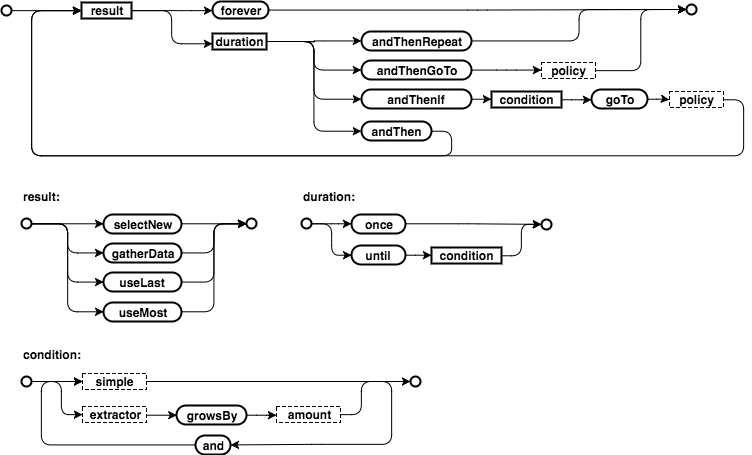
\includegraphics[width=140mm]{./img/policy_builder_chart.png}}}
	\caption{Syntax diagram of the \textit{policy builder} DSL.}
	\label{fig:policy_builder_chart}
\end{figure}

The policy built with \textit{policy builder} has always one main loop. Its definition starts with the first result that it emits: \textit{selectNew}, \textit{gatherData}, \textit{useMost} or \textit{useLast}. A result is always followed by a duration specifier, and another result. When we specify the sequence of results and their durations, we can end it by either closing the main loop (using \textit{andThenRepeat}), by transitioning to an external policy (using \textit{andThenGoTo}, leads to a policy out of the loop), or by using \textit{forever} as a duration for the last result, which limits the loop just this one result. In addition, it is possible to put a conditional transition to a policy out of the loop anywhere in between two results (using \textit{andThenIf}).

The conditions can be either simple functions accepting statistical data and returning a boolean value, or a \textit{growsBy} condition with a value extractor\footnote{A function that extracts a value of some type from the statistical data. Default implementations are provided for the basic fields.} and an amount. A simple condition is evaluated only once against current statistical data. In case of the \textit{growsBy} condition, the extractor is executed once at the beginning of the policy loop and its result is stored, and the condition evaluation consist of executing it and comparing current result to the stored one.

An example of a simple policy described using the \textit{policy builder} follows. It produces \textbf{GatherData} 50 times, then \textbf{SelectNew} 50 times, and then either loops forever on \textbf{UseLast}, if the streak is larger than 20, or repeats the whole process otherwise.

\lstset{style=Scala}
\begin{lstlisting}
val conditional: Policy = (
  gatherData until (totalRunCount growsBy 50)
  andThen selectNew until (totalRunCount growsBy 100)
  andThenIf ((stats: StatisticDataProvider) => stats.getStreakLength >= 20) goTo (useLast forever)
  andThenRepeat)
\end{lstlisting}

\subsection{Policies and groups}

One of the techniques for improving the selection process is grouping the history records using some input features, as described in \ref{subsec:grouping}. We will extend the grouping to function statistics and to the current policy. It means that the combined function needs to hold the policy and the statistical data for every group, and perform transitions and statistics updates separately.

The main advantage is the possibility to take faster decisions in some groups, using for example the \textit{Pause selection after streak} policy. When a function is significantly faster than the others for some category of inputs, the streak will build up fast within the group and the invocation for future inputs from such a group will require no selection and will be very quick, yielding correct results.

\subsection{Possible improvements}
\label{subsec:policy_improvements}

The policies were designed as a concept that is completely independent from the actual selection strategies and history analysis. One of the improvements that would require closer tying would be to allow the policies to choose the selection strategy, or to influence it somehow, by limiting it to a subset of data, etc. 

Another improvement that might seem useful is to let the policies analyze the whole history data. This would, however, mean a lot of additional overhead time when evaluating the policy, which is not desirable.
With a different approach, we could achieve the same thing by giving selection strategies a state that could involve their decision. The state would be managed by the combined function and it could even be the same state that is used by the policies. 

Next, a factor of combined certainty of all the selections of a specific function could be included in the statistical data. This factor could be aggregated from the selection results of the strategies that would support it (in the statistical test based strategies, it could be a p-value, strength of the test, or similar) and would serve as a decision factor for more complex policies.

%TODO - when do I need more data?
